
\section{Introduction}

%Array programming is the core abstraction behind many of the modern miracles of computing (e.g. neural networks, scientific simulation, database processing). 
Arrays are the most fundamental abstraction in computer science. Arrays and lists are often the first-taught datastructure
\cite[Chapter 2.2]{abelson_structure_1996}, \cite[Chapter 2.2]{knuth_art_1997}.
%
Arrays are also universal across programming languages, from their introduction
in Fortran in 1957 to present-day languages like Python
\cite{backus_fortran_1957}, keeping more-or-less the same semantics.
%
Modern array programming languages such as NumPy~\cite{harris_array_2020},
SciPy~\cite{virtanen_scipy_2020}, MatLab~\cite{moler_history_2020},
TensorFlow~\cite{abadi_tensorflow_2016}, PyTorch~\cite{paszke_pytorch_2019}, and
Halide~\cite{ragan-kelley_halide_2013} have pushed the limits of productive data
processing with arrays, fueling breakthroughs in machine learning, scientific
computing, image processing, and more.
% EASY CUT
%These frameworks have been the
%subject of extensive industry investment to enable performant implementations,
%and often operate at the peak capacity of the hardware they run on
%\cite{lo_roofline_2015}.

The success and ubiquity of arrays is largely due to their simplicity. 
%
Since their introduction, multidimensional arrays have represented dense, rectilinear,
integer grids of points. 
%
By \textbf{dense}, we mean that indices are mapped to value via a simple formula relating multidimensional space to linear memory.
%
Consequently, dense arrays offer extensive compiler optimizations and many convenient interfaces.
%
%This
%simplicity enables extensive interoperability, convenience layers, and
%optimizations by breaking the abstraction barrier between array representation
%and array storage.  
%
Compilers understand dense computations across many
programming constructs, such as for and while loops, breaks, parallelism,
caching, prefetching, multiple outputs, scatters, gathers, vectorization,
loop-carry-dependencies, and more. A myriad of optimizations have been developed for
dense arrays, such as loop fusion, loop tiling, loop unrolling, and loop
interchange.
%
However, while dense arrays are the easiest way to program for performance, the world is not all dense.

\begin{figure}
	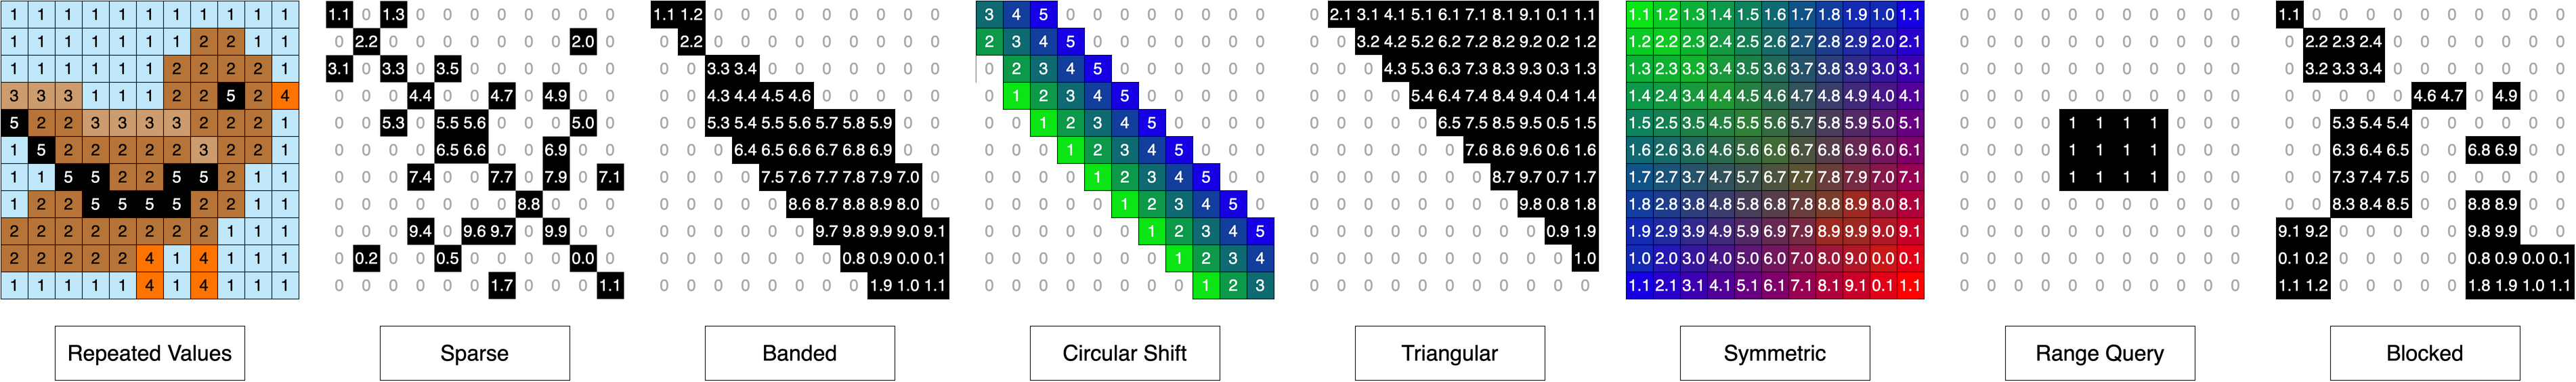
\includegraphics[width=\linewidth]{Structures-examples.png}
    \vspace{-12pt}
    \caption{A few examples of matrix structures arising in practice}
    \vspace{-8pt}
\end{figure}

Our world is full of structured data.
%
Sparse arrays (which store only nonzero elements) describe networks, databases, and simulations~\cite{abhyankarpetsc, bell2007lessons, mcauley2013hidden, balay2020petsc}.
%
Run-length encoding describes images and masks, geometry, and
databases (such as a list of transactions with the date field all the same)~\cite{shi2020column,golomb1966run}.
%
Symmetry, bands, padding, and blocks arise due to modeling choices in scientific computing (e.g., higher order FEMs) as well as in intermediate structures in many linear solvers (e.g., GMRES)~\cite{ded, saad2003iterative, o2009scientific}.
%
In the context of machine learning, combinations of sparse and blocked matrices are increasingly under consideration~\cite{dao2022monarch}.
%
Even complex operators can be expressed as structured arrays.
%
For example, a convolution with a filter can be expressed as a matrix multiplication
with the toeplitz matrix of all the circular shifts of the filter~\cite{sze2017efficient}.

%
\textbf{Currently, support for structured data is fragmented and incomplete}.
%
Experts must hand write variations of even the simplest kernels, like matrix
multiply, for each data structure/data set and architecture to get performance.
%
Implementations must choose a small set of features to support well, resulting
in a compromise between \textbf{program flexibility} and \textbf{data structure
flexibility}.
%
Hand-written solutions are collected in diverse libraries like
MKL, OpenCV, LAPACK or SciPy~\cite{ bradski2000opencv, anderson1999lapack, virtanen2020scipy, psarras2022linear}. 
%
However, libraries will only ever support a subset of
programs on a subset of data structure combinations.
%
Even the most advanced
libraries, such as the GraphBLAS, which support a wide variety of sparse
operations over various semi-rings always lack support for other features, such
as tensors, fused outputs, or runs of repeated values~\cite{bulucc2017design, mattson2019lagraph}.
%
While dense array
compilers support an enormous variety of program constructs like early break and
multiple left hand sides, they only support dense arrays~\cite{ragan-kelley_halide_2013,grosser2012polly}.  
%
Special-purpose
compilers like TACO~\cite{kjolstad_tensor_2019}, Taichi~\cite{hu_taichi_2019}, StructTensor~\cite{ghorbani2023compiling}, or CoRa~\cite{fegade_cora_2022} which support a select subset of structured data
structures (only sparse, or only ragged arrays) must compromise by greatly
constraining the classes of programs which they support, such as tensor
contractions.
%
This trade-off is visualized in Tables \ref{tab:features} and \ref{tab:data_structures}.
%

\newcommand*\rot{\rotatebox{90}}

\begin{table}[b!]
\vspace{-12pt}
\noindent
\flushleft
\begin{minipage}[t]{.49\textwidth}
  \scriptsize
  \begin{tabular}{l|cccccc}
  \textbf{Feature / Tool} & \rothead{Halide} & \rothead{Taco} & \rothead{Cora} & \rothead{Taichi} & \rothead{Stur} & \rothead{Finch} \\
  \hline
  Einsums/Contractions & \checkmark & \checkmark & \checkmark & \checkmark & \checkmark & \checkmark \\
  % High-Level API           &            & \checkmark &            &            &            & \checkmark \\
  % Automatic API Fusion     &            &            &            &            &            & \checkmark \\
%  Parallelism             & \checkmark & \checkmark & \checkmark & \checkmark&           & \checkmark \\
  Multiple LHS             & \checkmark &            & \checkmark & \checkmark &            & \checkmark \\
  Affine Indices           & \checkmark &            &            & \checkmark & \checkmark & \checkmark \\
  Recurrence               & \checkmark &            &            &            &            &           \\
  If-Conditions and Masks  & \checkmark & \checkmark &            & \checkmark &            & \checkmark \\
  Scatter Gather           & \checkmark &            &            & \checkmark &            &\checkmark \\
  Early Break              &            & \checkmark &            & \checkmark &            &\checkmark \\
  Unrestricted Read/Write              &    \checkmark        &  &            &  &            &  \\
  \end{tabular}
  \caption{Control flow support across various tools.}
  \label{tab:features}
\end{minipage} 
\begin{minipage}[t]{.49\textwidth}
  \flushright
  \scriptsize
  \begin{tabular}{l|cccccc}
  \textbf{Feature / Tool} & \rothead{Halide} & \rothead{Taco} & \rothead{Cora} & \rothead{Taichi} & \rothead{Stur} & \rothead{Finch} \\
  \hline
  Dense                    & \checkmark & \checkmark & \checkmark & \checkmark & \checkmark & \checkmark \\
  Padded                   & \checkmark &            &            &            &            & \checkmark \\
  One Sparse Operand              &            & \checkmark &            & \checkmark &            &\checkmark \\
  Multiple Sparse  Operands                 &            & \checkmark &            &            &            &\checkmark \\
  Run-length               &            &            &            &            &            & \checkmark \\
  Symmetric                &            &            &            &            & \checkmark & \checkmark \\
  Regular Sparse Blocks    &            & \checkmark &            &            &            & \checkmark \\
  Irregular Sparse Blocks  &            &            &            &            &            &\checkmark \\
  Ragged                   &            &            & \checkmark &            &            & \checkmark \\
  \end{tabular}
  \caption{Data structure support across various tools.  Finch supports \textbf{both} complex programs and complex data structures.}
  \label{tab:data_structures}
\end{minipage}
\vspace{-24pt}
\end{table}


%
Prior implementations are incomplete because the abstractions they use are tightly coupled with the specific data structures that they support.
%
For example, TACO merge lattices represent boolean logic over sets of non-zero values on an integer grid~\cite{kjolstad_tensor_2017}.
%
The polyhedral model allows various compilers to represent dense computations on affine regions~\cite{grosser2012polly}.
%
Taichi enriches single static assignment form with a specialized instruction for accessing only a single sparse structure, but it supports more control flow ~\cite{hu_taichi_2019}.
These systems tightly couple their control flow to narrow classes of data structures to avoid the challenges that occur when we intersect complex control flow with structured data. There are two challenges:
%writing efficient code over structured data


\textbf{Optimizations are specific to the indirection and patterns in data structures}: 
%
These structures break the simple mapping between array elements and where they are stored in memory.
%
For example, sparse arrays store lists of which coordinates are nonzero, whereas run-length-encoded arrays map several pixels to the same color value. 
%
These zero regions or repeated regions are optimization opportunities, and we must adapt the program to avoid repetitive work on these regions by referencing the stored structure.

\textbf{Performance on structured data is highly algorithm dependent}: The landscape of implementation decisions is dramatically unpredictable. 
%
For example, the asymptotic performance of sparse matrix multiplication can be impacted by the distribution of nonzeros, the sparse format, and the loop order~\cite{ahrens2022autoscheduling, zhang2021gamma}. 
%For example, sparse kernels don't need to compute on zeros, but this means that the precise input nonzero patterns act as computational filters, affecting the runtime as they interact with each other and the implementation.
This means that performance engineering for such kernels requires the exploration of a large design space, changing the algorithm as well as the data structures.



\textbf{In this work, we propose a new programming language, Finch, which supports \textit{both} flexible control flow and diverse data structures.}
%
Finch facilitates a programming model which resolves the challenges of computing over structured arrays by \textbf{combining control flow and data structures into a common representation where they can be co-optimized}.
%
In particular, Finch automatically specializes the control flow to the data so that performance engineers can focus on experimenting with many algorithms.
%
Finch supports a familiar programming language of loops, statements, if conditions, breaks, etc., over a wide variety of array structures, such as sparsity, run-length-encoding, symmetry, triangles, padding, or blocks. 
%
This support would be useless without the appropriate level of structural specialization; Finch reliably utilizes the key properties of structure, such as structural zeros, repeated values, or clustered non-zeros.
%

As an example, a programmer might explore different ways to intersect only the even integers of two lists (represented as sparse vectors with sorted indices). The control flow here is only useful if the first example differs from the next two in that it actually selects only even indices as the two integer lists are merged and different from the last in that it does not require another tensor:
%The Finch compiler uses the structure of the data to generate efficient implementations of these programs.

%\teo{Proposed new paragraph:}
%\teo{Add: }
%\teo{We don't propose to solve these problems automatically, but we do propose a new programming language where these issues are solvable, by virtue of the precise manner in which we combine structured data and control flow.}
%
%\teo{Our language, Finch, combines structured data and control flow in a predictable manner by lowering both of them into a single abstraction} Looplets~\cite{ahrens_looplets_2023}, which combines structured iterators into a single control flow that only produces the relevant portions of the output.}
%
%\teo{For example, if a programmer wanted to merge the even indices of two sorted arrays, a programmer could represent by point-wise multiplying two sparse vectors to produce another sparse vector and then set the even indices two zero or the programmer could only point-wise multiply the two sparse vectors under an if condition that selects even indices. (This crucial part needs improvement)}
%
%\teo{Via index expressions, multiple levels of loops and tensors, and more complex filtering expressions, we can imagine many variation of this problem with fine grained distinctions about when various operations are performed.}


\begin{minipage}{0.25\linewidth}
\begin{minted}{julia}
     for i = _
         if i % 2 == 0
             c[i]=a[i]*b[i]
         end
     end
\end{minted}
\end{minipage}%
\begin{minipage}{0.25\linewidth}
\begin{minted}{julia}
     for i = _
         if i % 2 == 0
             ap[i] = a[i]
         end
     end
     for i = _
         c[i] = ap[i] * b[i]
     end
\end{minted}
\end{minipage}%
\begin{minipage}{0.25\linewidth}
\begin{minted}{julia}
     for i = _
         cp[i] = a[i] * b[i]
     end
     for i = _
         if i % 2 == 0
             c[i] = cp[i]
         end
     end
\end{minted}
\end{minipage}%
\begin{minipage}{0.25\linewidth}
\begin{minted}{julia}
     for i = _
        if i % 2 == 0
            f[i] = 1
        end
     end
     for i = _
        c[i] = a[i] * b[i] * f[i]
     end
\end{minted}
\end{minipage}%

\subsection{Contributions}


\begin{enumerate}
\item More complex array structures than ever before. We are the first to extend level-by-level hierarchical descriptions to capture banded, triangular, run-length-encoded, or sparse datasets, and any combination thereof.
%
We have chosen a set of level formats that completely captures all combinations of relevant structural properties (zeros, repeated values, and/or blocks).
%
Although many systems (TACO, Taichi, SPF, Ebb)~\cite{chou2018format,  hu_taichi_2019, strout2018sparse, bernstein2016ebb} feature a flexible structure description, our level abstraction is more capable and extensible because it uses Looplets \cite{ahrens_looplets_2023} to express the structure of each level. 
%
\item A rich structured array programming language with for-loops and complex control flow constructs at the same level of productivity of dense arrays. 
%
To our knowledge, the Finch programming language is the first to support if-conditions, early breaks, and multiple left hand sides over structured data, as well as complex accesses such as affine indexing or scatter/gather of sparse or structured operands.
%
\item A compiler that specializes programs to data structures automatically, facilitating an expressive language that makes it easier to search the complex space of algorithms and data structures. Finch reliably utilizes four key properties of structure, such as structural zeros, repeated values, clustered non-zeros, and singletons.
%
\item Our compiler is highly extensible, evidenced by the variety of level formats and control flow constructs that we implement in this work.
%
For example, Finch has been extended to support real-valued array indices with continuous arrays \cite{won2024continuous}.
%
\item We evaluate the efficiency, flexibility, and expressibility of our language in several case studies on a wide range of applications, demonstrating speedups over the state of the art in classic operations such as spmv ($2.51\times$) and spgemm ($1.25\times$), to more complex applications such as graph analytics ($3.53\times$, reducing lines of code by $4\times$ over GraphBLAS), image processing ($19.5\times$), and the Python Array API ($28\times$).
%We also demonstrate how Finch can fuse high-level operations to achieve a significant speedup over non-fused kernels. Additionally, as a case study, a high-level array programming language and fusion interface for operations such as map, broadcast, or reduce that can be compiled to efficient code using the previous loop-level abstractions.
%\item A complete set of level formats for expressing data patterns hierarchically in FiberTree-style decompositions. The first such set of formats to efficiently capture banded, triangular, run-length-encoded, or sparse-run-length-encoded datasets. The formats capture many use cases, from random updates to sequential construction.
%\item The Finch array language, mirroring simple for-loops with imperative code blocks and if-conditions. The first array programming language for the above data formats to support multiple outputs, affine indexing, and imperfectly-nested loops.
%\item Tensor lifecycles, a simple constraint on tensor reads and writes that elegantly restricts Finch programs to avoid complex data dependencies, and enables tensor polymorphism by providing implementers with well-defined functions to overload.
%\item Wrapper Tensors which modify existing datastructures and recombine them to support new patterns, such as affine indexing, padding, transposition, and slicing.
%\item Wrapper Levels which modify existing datastructures and enabling complex features such as atomic updates or contiguous versus separate allocation.
%\item We define the first mappings from the existing pydata/sparse array api high-level operations to low level finch notation
%\item <Performance Contributions>

\end{enumerate}

This advances the state-of-the-art over the looplets work \cite{ahrens_looplets_2023}. While Looplets presented a way to merge iterators over multiple single dimensional structures, we go further by combining single-dimensional looplets into multi-dimensional tensors and operating on them in a programming language with fully-featured control flow.
